%research area
Infrastructure systems play a critical role in the ability of a region to recover after an earthquake; damages can have massive social and economic consequences~\cite{chang_measuring_2001,chang_evaluating_2003,rose_business_2002,araneda_lessons_2010}.  Researchers conventionally assess the seismic risk of an infrastructure system using event-based methods: primarily by modeling the seismic hazard using simulated scenario earthquakes \cite[e.g.,][]{romero_seismic_2010,rokneddin_bridge_2013,chang_measuring_2001} or using Monte Carlo simulation (MCS) of various earthquake events (defined by source and magnitude) as part of an event-based probabilistic loss estimation model \cite[e.g.,][]{bommer_development_2002,grossi_catastrophe_2005,crowley_modelling_2006,stergiou_treatment_2006,shiraki_system_2007,jayaram_efficient_2010}. 
%An event-based probabilistic loss estimation model samples relevant random variables like earthquake magnitude from corresponding distributions and each time evaluates what the impact is on the infrastructure network. The results are aggregated to estimate seismic risk. 
%why important
With a better understanding of risk, steps toward risk mitigation can be taken such as insuring against supply chain disruptions or retrofitting water pipelines or bridges.

%%recent advances (I'm thinking clustering by Nirmal and work by Han and Davidson)
Event-based methods are the standard approaches for assessing infrastructure seismic risk  because the link between earthquake ground motions and network performance measures is often not possible to express in a closed form.  Event-based methods involve probabilistically generating ground-motion intensity maps considering rupture scenarios that could occur in the region. Conditioned on the ground-motion intensity, damage is probabilistically sampled at all network components of interest. %In the event-based method, many earthquakes are simulated to create a \emph{synthetic earthquake catalog}, which are also called a set of ground-motion intensity maps. damage state of different system components
Since various random variables including magnitude, rupture location, and damage states of system components must be sampled, there is an infinite set of possible damage maps to evaluate. At the same time, computing the earthquake impacts on the infrastructure system, whose numerical results we will call \emph{network performance measures}, often requires computationally expensive calculations. Thus, to make the event-based method computationally feasible, researchers must choose a reduced set of damage maps and associated ground-motion intensity maps to model.  
%Directly solving the subset selection problem by evaluating the error with relevant exceedance rates for each possible combination of $\binom mk$ maps and each associated occurrence rate is not feasible unless $m$ and $k$ are small and the space for the occurrence rates is artificially discretized and limited. 

%%recent advances (I'm thinking clustering by Nirmal and work by Han and Davidson)
Previous work on efficient simulation of events draws on statistical techniques. For example, since the earthquakes of greatest interest tend to be very rare, importance sampling is often used to minimize the number of events to evaluate by preferentially sampling important events, such as large magnitude earthquakes~\cite{stergiou_treatment_2006}.  Jayaram and Baker \cite{jayaram_efficient_2010} expanded on the importance sampling of magnitudes to also importance sample within-event residuals and then used K-Means clustering, a common clustering algorithm, to further reduce the number of ground-motion intensity maps. For a case study, Han and Davidson \cite{han_probabilistic_2012}, however, found higher errors between hazard estimates using the  clustering method and numerical integration results, than between their proposed optimization method  and numerical integration results. 
%Most recently, an optimization-based technique has been proposed to select damage maps, but the work is limited to a single ground-motion intensity scenario; the optimization formulation does not explicitly consider consistency with the input distributions of the ground-motion intensity or network performance~\cite{gearhart_optimization-based_2014}.
%problem/motivation/contribution (I'm thinking talking about issues with clustering and then talking about neither explicitly consider KPI's
In summary, no previous work evaluates consistency with the joint distribution of ground-motion intensity or the exceedance rates of network performance measures, which is the application of interest here, when selecting a subset of damage and ground-motion intensity maps.


%%mega-point
Here we show a computationally efficient method for selecting a subset of damage maps, corresponding ground-motion intensity maps, and associated occurrence rates using optimization that reasonably estimates the full distribution of a target performance measure and the ground-motion intensity.
 %to enable a more accurate and efficient probabilistic infrastructure network risk assessment.
%approach
%%method overview
From a set of candidate damage and ground-motion intensity maps and corresponding realizations of network performance, the optimization problem involves choosing a reduced set of damage and ground-motion intensity maps and associated annual rates of occurrence that minimizes the differences between the marginal ground-motion intensity and network performance loss exceedance curves of this set and an extensively-sampled baseline set over a range of return periods of interest. The optimization procedure implicitly includes the joint distribution of the ground-motion intensity via the network performance measure. 

Conceptually, an event-based framework estimates a loss exceedance curve by the superposition of each event's loss exceedance curve (of a rectangular block-like form, because this ``curve'' corresponds to only one value and occurrence rate) (top row of Figure~\ref{fig:blocks}); the proposed optimization procedure selects a subset of these ``blocks'', which are re-sized because of the new annual occurrence rates from the optimization, to stack together for a new estimated loss exceedance curve (bottom row of Figure~\ref{fig:blocks}).


\begin{figure*}[h]
    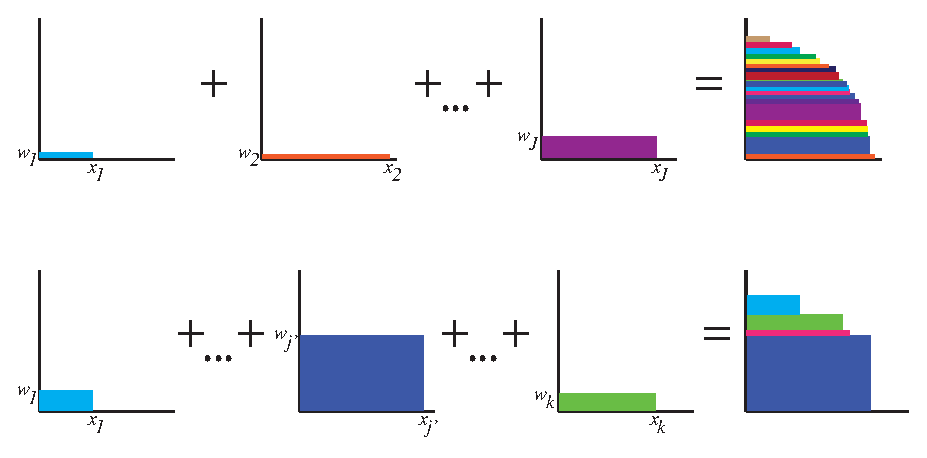
\includegraphics[width=\textwidth]{../FIGS/subset_blocks.eps} 
\caption{Conceptual depiction of loss exceedance curves from an event-based framework for a hypothetical example. For all subfigures, the X axis is \emph{$X$ = Performance measure} and the Y axis is the \emph{Annual rate of exceedance, $\lambda_{X>x}$}. The top row corresponds to an extensively-sampled event set including corresponding ground-motion intensity and damage maps. The bottom row corresponds to a subset of $k$ maps selected with the proposed optimization-based method, including re-weighting the occurrence rates, $w_{j'}$, of each map.}
\label{fig:blocks}
\end{figure*}

%more approach?
 To enable this optimization-based approach, we introduce two classes of network performance measures, proxy measures and target measures. The optimization procedure uses a proxy measure, since proxy measures ``serve as indirect measures of a given variable or process and are often used because of relative ease of measurement or understanding"~\cite{mckay_metric_2010}.  In contrast, target performance measures may be very computationally expensive. We choose a proxy performance measure to represent the target performance measure by combining ``soft'' knowledge, such as engineering experience, and an empirical method. Since the considered proxy network performance measure depends on the joint distribution of the ground-motion intensity, the proxy measure provides additional assurance that not only the target performance measure, but also the joint distribution of the ground-motion intensity, will be reasonably estimated. 
% 
%  help capture the joint distribution of the ground-motion intensity, because correlated losses usually correspond to high losses in network performance in contrast to independent component losses. Second, proxy measures can be chosen to be more strongly correlated to the target measure than the ground-motion intensity either by ``soft'' knowledge, such as engineering experience, or by an empirical method. %For example, if network failures result from component failures, this information can be used to choose a proxy measure related to component failures, which is a more direct relation to the network performance than the ground motion intensity. Alternatively, by using empirical correlation coefficients and limited tests, as will be discussed, we can empirically choose a proxy measure more correlated to the target performance measure than the ground motion intensity measure alone. 
 Finally, we describe a series of checks, a preliminary version of which we proposed in~\cite{miller_framework_2014}, to tune the model parameters to produce a final set of damage and ground-motion intensity maps. We also test that the final set is reasonably representative of an extensively-sampled baseline set of maps across various dimensions.
 
%%extensions (I'm thinking of discussing what the user would have and why I have correct answers)
To illustrate the proposed method, we assess the seismic risk to the San Francisco Bay Area road network with an event-based probabilistic loss estimation model. We show that by choosing maps based on spectral acceleration and a proxy performance measure (percentage of bridges damaged region-wide) in the objective function, we achieve low error for a more computationally intensive target performance measure (average percentage change in morning commute travel time). 
%gist of results

%significance
%This framework saves the researcher significant computational time in evaluating the seismic risk of infrastructure systems using event-based methods. Given the greater computational efficiency of our approach over other methods, the optimization framework enables better agreement between a risk estimate one would obtain from a full Monte Carlo analysis and some computationally tractable set of maps. 
Although the proposed framework requires formulating the optimization problem for the desired application and calculating proxy network performance measures for selecting a subset of damage and ground-motion intensity maps, the time invested in map selection is greatly outweighed by the expected savings in overall computational time for the risk analysis. The result is a more accurate and efficient probabilistic infrastructure network risk assessment.




